Attack trees are a type of tree based graphical model used in
analyzing the threat potential of secure systems.  They were
popularized by Bruce Schneier \cite{Schneier:1999} at the NSA and they
were found to be affective at analyzing both physical and virtual
secure systems.  An attack tree represents all possible ways to
accomplish a particular attack on a system.  The root of the tree is
the over all goal, and then each child node represents a refinement of
the overall goal.  The leafs are particular attacks needed to
accomplish the goal of the tree.  An example attack tree for attacking
an ATM can be found in Figure~\ref{fig:atm-tree1}.

In this paper attack trees have three types of branching nodes:
and-node, or-nodes, and sequence-nodes.  And-nodes are depicted
graphically by drawing a horizontal line linking the children nodes.
This type of node represents a set of attacks that all must be
executed, but there is no particular order on which must be executed
first. Similarly, sequence-nodes are depicted by a horizontal arrow
linking the children nodes.  These nodes represent ordered execution
of attacks.  Finally, the remaining nodes are or-nodes which represent
a choice between attacks.  This formalization of attack trees is known
as SAND attack trees and were introduced by Jhawar
et. al~\cite{Jhawar:2015}.

The way in which we describe attack trees suggests that they should be
considered as describing a process in terms of smaller processes.
Then each leaf of an attack tree represents a process -- an attack --
that must be executed to reach the overall goal.  Branching nodes are
then operators of process algebra.  Thus, an attack tree is a process
tree representing an attack.

Until recently attack trees have been primarily a tool without a
theoretical foundation.  This has become worrisome, because several
projects have used them to asses the security of large scale systems.
Therefore, a leading question regarding attack trees is, what is a
mathematical model of attack trees?  There have been numerous proposed
answers to this question.  Some examples are propositional logic,
multisets, directed acyclic graphs, source sink graphs (or
parallel-series pomsets), Petri nets, and Markov processes.

Give that there are quite a few different models one can then ask, is
there a unifying foundation in common to each of these proposed
models?  Furthermore, can this unifying foundation be used to further
the field of attack trees and build new tools for conducting threat
analysis?  This paper contributes to the answer of these questions.
Each of the proposed models listed above have something in common.
They can all be modeled in some form of a symmetric monoidal category
\cite{Tzouvaras:1998,Brown:1991,Fiore:2013,FrancescoAlbasini2010}.
That is all well and good, but what can we gain from monoidal
categories?

Monoidal categories are a mathematical model of linear logic as
observed through the beautiful Curry-Howard-Lambek correspondence
\cite{Mellies:2009}.  In linear logic every hypothesis must be used
exactly once, and hence, if we view a hypothesis as a resource, then
this property can be stated as every resource must be consumed.  This
is an ideal setting for reasoning about processes like attack trees.

Multisets and Petri nets both capture the idea that the nodes of an
attack tree consist of the attack action and the state -- the
resource -- of the system being analyzed. As it turns out, linear
logic has been shown to be a logical foundation for multisets
\cite{Tzouvaras:1998} and Petri Nets \cite{Brown:1991}.  Thus, linear
logic has the ability to model the state as well as attack actions of
the goals of an attack tree.  

In this paper\footnote{This material is based upon work supported by
  the National Science Foundation CRII CISE Research Initiation grant,
  ``CRII:SHF: A New Foundation for Attack Trees Based on Monoidal
  Categories``, under Grant No. 1565557.} we introduce a new logical
foundation of SAND attack trees in intuitionistic linear logic.  This
new foundation is based on a new logic called the Attack Tree Linear
Logic (ATLL).

\begin{wrapfigure}{r}{0.5\textwidth}
  \vspace{-45px}
  \begin{center}
    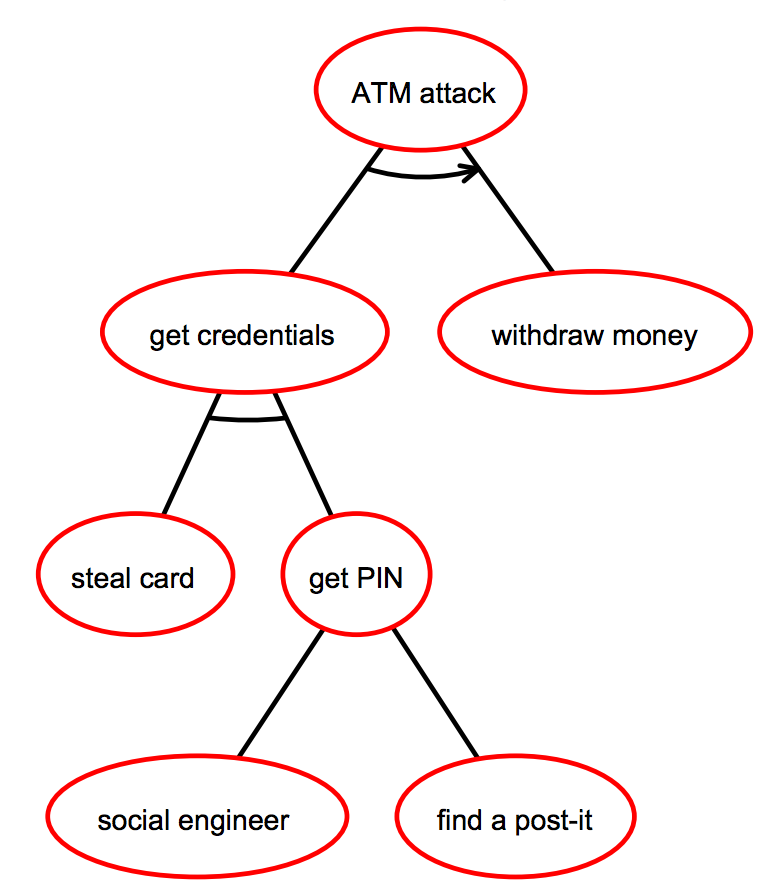
\includegraphics[scale=0.210]{ATM-Tree1}
  \end{center}  
  \label{fig:atm-tree1}
  \caption{Attack Tree for an ATM attack from Figure~1 on page 2 of Kordy et al.~\cite{Kordy2017}}
  \vspace{-55px}
\end{wrapfigure}
In ATLL (Section~\ref{sec:the_attack_tree_linear_logic_(atll)}) attack
trees are modeled as linear formulas where base attacks are atomic
formulas, and each branching node corresponds to a binary logical
connective.  Consider the attack tree for an ATM attack from
Figure~\ref{fig:atm-tree1}.  We can model this attack tree as a
formula in ATLL as follows:
\[
\begin{array}{lll}
  \ATLLnt{B_{{\mathrm{1}}}} := \text{``steal card''}\\
  \ATLLnt{B_{{\mathrm{2}}}} := \text{``social engineer''}\\
  \ATLLnt{B_{{\mathrm{3}}}} := \text{``find a post-it''}\\
  \ATLLnt{B_{{\mathrm{4}}}} := \text{``withdrawal money''}\\
  \ATLLnt{T_{{\mathrm{1}}}} := \ATLLsym{(}  \ATLLnt{B_{{\mathrm{1}}}}  \odot  \ATLLsym{(}  \ATLLnt{B_{{\mathrm{2}}}}  \sqcup  \ATLLnt{B_{{\mathrm{3}}}}  \ATLLsym{)}  \ATLLsym{)}  \rhd  \ATLLnt{B_{{\mathrm{4}}}}
\end{array}
\]
Each $\ATLLnt{B_{\ATLLmv{i}}}$ is an atomic formula, parallel conjunction -- and-nodes
-- of attack trees is denoted by $\ATLLnt{T_{{\mathrm{1}}}}  \odot  \ATLLnt{T_{{\mathrm{2}}}}$, choice between
attacks -- or-nodes -- by $\ATLLnt{T_{{\mathrm{1}}}}  \sqcup  \ATLLnt{T_{{\mathrm{2}}}}$, and sequential conjunction of
attacks -- sequence-nodes -- by $\ATLLnt{T_{{\mathrm{1}}}}  \rhd  \ATLLnt{T_{{\mathrm{2}}}}$.  Parallel conjunction
and choice are both symmetric, but sequential conjunction is not.  Now
that we can model attack trees as formulas we should be able to use
the logic to reason about attack trees.

Reasoning about attack trees corresponds to proving implications
between them.  In fact, every equation from Jhawar et al.'s
work on attack trees with sequential conjunction \cite{Jhawar:2015}
can be proven as an implication in ATLL.  Consider a second attack
tree from Figure~\ref{fig:atm-tree2}.
\begin{figure}
  \begin{center}
    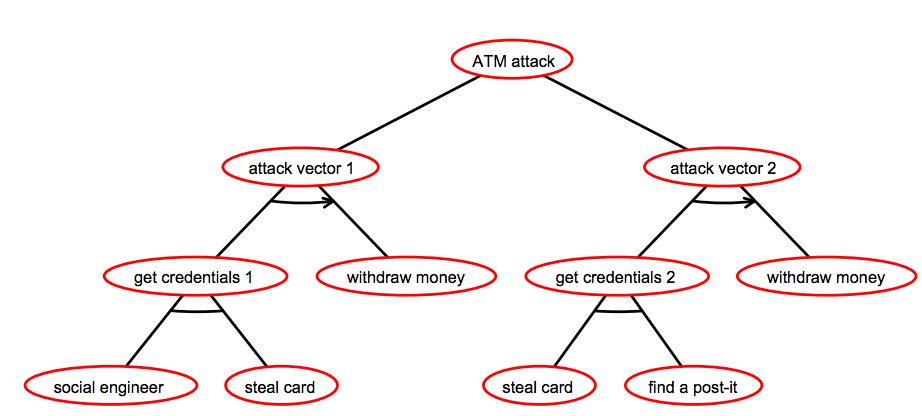
\includegraphics[scale=0.35]{ATM-Tree2}
  \end{center}
  \caption{Canonical Attack Tree for an ATM attack from Figure~2 on page 3 of Kordy et al.~\cite{Kordy2017}}
  \label{fig:atm-tree2}
\end{figure}
We can model this attack tree as a formula in ATLL as well (the base
attacks are the same):
\[
\begin{array}{lll}
  \ATLLnt{T_{{\mathrm{2}}}} := \ATLLsym{(}  \ATLLsym{(}  \ATLLnt{B_{{\mathrm{1}}}}  \odot  \ATLLnt{B_{{\mathrm{2}}}}  \ATLLsym{)}  \rhd  \ATLLnt{B_{{\mathrm{4}}}}  \ATLLsym{)}  \sqcup  \ATLLsym{(}  \ATLLsym{(}  \ATLLnt{B_{{\mathrm{1}}}}  \odot  \ATLLnt{B_{{\mathrm{3}}}}  \ATLLsym{)}  \rhd  \ATLLnt{B_{{\mathrm{4}}}}  \ATLLsym{)}
\end{array}
\]
The attack trees $\ATLLnt{T_{{\mathrm{1}}}}$ and $\ATLLnt{T_{{\mathrm{2}}}}$ represents the same attack, and
this can be proven in ATLL by showing that $\ATLLnt{T_{{\mathrm{1}}}}  \multimapboth  \ATLLnt{T_{{\mathrm{2}}}}$ where
$ \multimapboth $ denotes bi-implication.  The proof holds by using the
distributive rules for choice.

Modeling attack trees in linear logic has a number of benefits.
First, it connects attack trees back to logic, but in elegant and
simple way.  Kordy et al.~\cite{Kordy2010,Kordy:2012} proposed that
attack trees be modeled in propositional logic, but in this model
attacks can be freely duplicated and contracted which goes against the
process nature of an attack tree.  However, linear logic restores this
natural interpretation without loosing the process interpretation of
attack trees and without having to resort to complicated notation
unlike models similar to the situation calculus \cite{Samarji2013}.
By connecting attack trees to logic we can also tap into the long
standing research and development of automation, for example, SAT,
SMT, proof search, etc.  Finally, by connecting to logic we also
connect to the theory of statically typed functional programming
through the Curry-Howard-Lambek correspondence which will allow for
the development of a programming language that can be used to certify
the correctness of attack trees and the analysis performed using them.
In particular, we can use ATLL to design a functional scripting
language for the definition of attack trees that has the same
semantics as attack trees.

Before introducing ATLL we given several new logical models of attack
trees starting in
Section~\ref{sec:a_quaternary_semantics_for_sand_attack_trees} with a
very basic truth table semantics.  Then we lift this semantics into a
semantics of attack trees based on lineales in
Section~\ref{sec:lineale_semantics_for_sand_attack_trees}, but this
can be further lifted into a dialectica model which ATLL is based
(Section~\ref{sec:dialectica_semantics_of_sand_attack_trees}).

\textbf{Contributions.}  This paper offers the following
contributions:
\begin{itemize}
\item The first simple truth table semantics of SAND attack trees,
\item The first categorical model of attack trees in dialectica
  categories,
\item The Attack Tree Linear Logic (ATLL): a new intuitionistic linear
  logic for the specification and analysis of attack trees.

\item Horne et al.~\cite{horne2017semantics} propose to model attack
  trees in linear logic as well, but their logic is based on classical
  linear logic, and does not support full distribution of sequential
  conjunction over choice, while ATLL does.
\end{itemize}

Every section except
Section~\ref{sec:the_attack_tree_linear_logic_(atll)} has been
formalized in the Agda proof assistant\footnote{The Agda formalization
  can be found here
  \url{https://github.com/MonoidalAttackTrees/ATLL-Formalization}}.
Furthermore, all of the syntax used in this paper was formalized using
OTT~\cite{Sewell:2010}.
